\subsection{Choix Techniques}

\begin{frame}{Choix du langage de programmation}
	\begin{block}{C++}
  	\begin{itemize}
    	\item rapidité d'éxecution
    	\item langage à objets
    	\item connaissance du langage
    	\item langage très répandu
  	\end{itemize}
	\end{block}
\end{frame}

\begin{frame}{Utilisation d'un gestionnaire de version}
	\begin{block}{git - the stupid content tracker}
  	\begin{itemize}
    	\item sauvegarde
    	\item partage
    	\item mise en commun
  	\end{itemize}
	\end{block}
\end{frame}

\subsection{Structures}
\begin{frame}{Représentation du problème de flot maximum}
	\begin{block}{Réseau de transport}
  	\begin{itemize}
    	\item Graphe orienté et pondéré
    	\item une source
    	\item un puits
  	\end{itemize}
	\end{block}
	\begin{block}{Graphe d'écarts}
  	\begin{itemize}
    	\item Graphe orienté et pondéré
  	\end{itemize}
	\end{block}
\end{frame}


\begin{frame}{Représentation du problème de flot maximum}
	\begin{block}{Graphe de couches}
  	\begin{itemize}
    	\item Graphe orienté et pondéré
  	  \item un tableau de listes de sommets (chaque liste représente une couche)
  	\end{itemize}
	\end{block}
\end{frame}

\begin{frame}{Diagramme de classes}
	\begin{figure}
	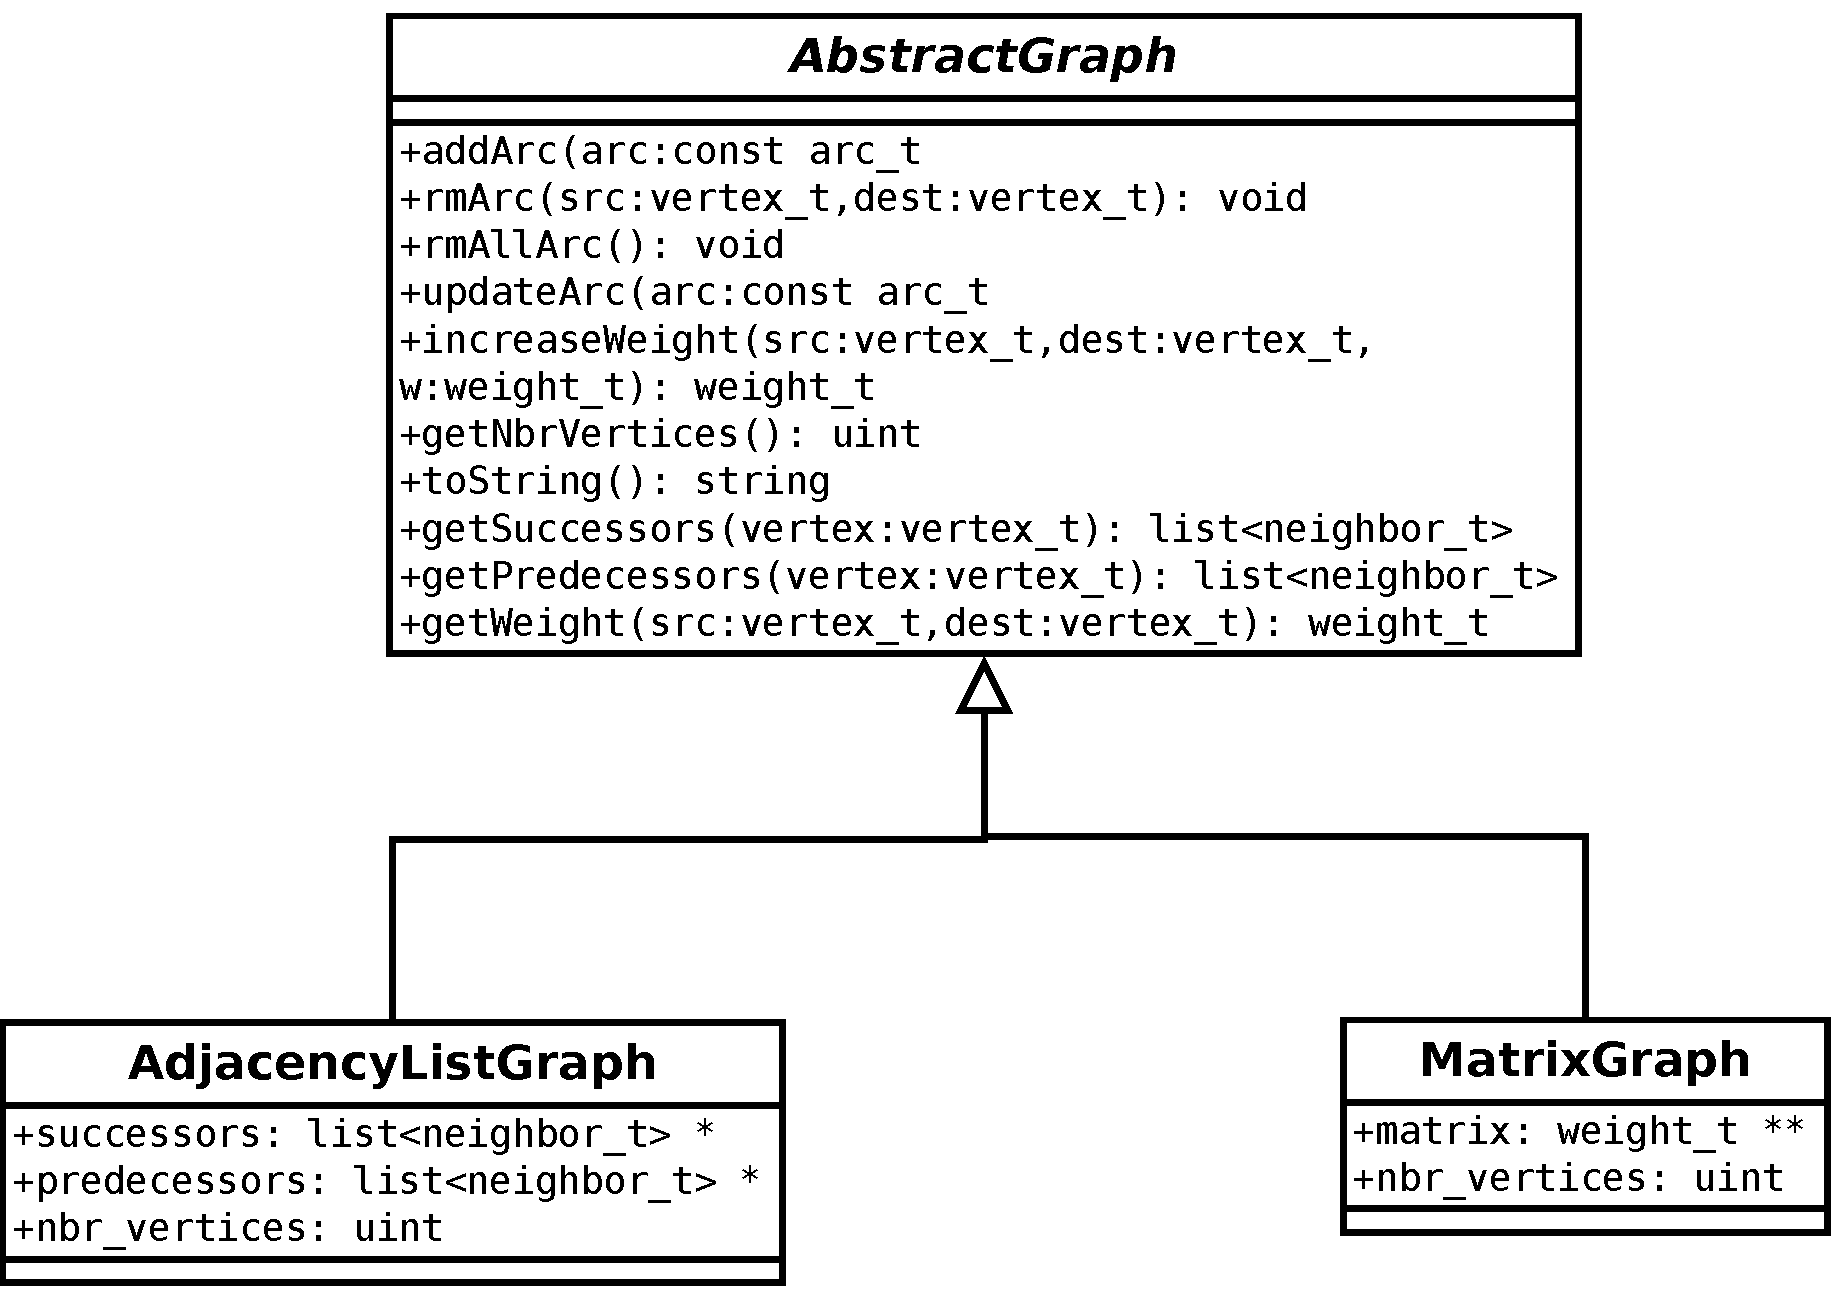
\includegraphics[width=0.8\textwidth]{img/diag_class.pdf}
	\end{figure}
	% Classe abstraite pour s'abstraire dans les algos des structures de données
\end{frame}

\subsection{Mise en oeuvre des algorithmes}
\begin{frame}{Génération de réseaux de transport aléatoires}
	\begin{block}{Deux stratégies}
  	\begin{itemize}
  		\item Tirage aléatoire de deux sommets
  		\item Génération de tous les arcs possibles et tirage d'un arc
  	\end{itemize}
	\end{block}
\end{frame}

\begin{frame}{Edmonds-Karp}
	 \begin{itemize}
  	\item Recherche du plus court chemin en nombre d'arcs par un parcours en largeur
  \end{itemize}
\end{frame}

\begin{frame}{Dinic}
	 \begin{itemize}
	 	\item Génération du graphe de couche par un parcours en largeur en stockant l'ensemble des parents.
  	\item Complexité de l'accès au prédécesseur dans le graphe de couche pour le calcul du flot bloquant
  \end{itemize}
\end{frame}